\subsection{Algorithmus}\label{subsec:algorithmus}

\paragraph{AVL-Bedingung}
Ein AVL-Baum ist ein Binärbaum, der die zusätzliche Eigenschaft besitzt, dass
die Balance, die als die Differenz der Höhe $h$ der beiden
Teilbäume definiert ist (siehe Formel~\ref{eq:balance}), bei jedem Knoten maximal 1 beträgt.
Diese Eigenschaft wird AVL-Bedingung genannt.
Dabei ist die Höhe analog zum regulären Binärbaum definiert (siehe~\ref{eq:equation}).

\begin{equation}
    bal(k) = h(T_r) - h(T_l)\label{eq:balance} \in \{-1,0,1\}
\end{equation}
\begin{equation}
    h(k) = max(h(T_l), h(T_r))\label{eq:equation}
\end{equation}
Durch diese Bedingung wird sichergestellt, dass der Baum zu jedem Zeitpunkt
balanciert ist und somit das in der Einleitung beschriebene Problem der
schlechten Laufzeit des Binärbaumes durch Entartung nicht auftreten kann.

\paragraph{Rebalancierung}
Nach dem Einfügen und Löschen von Elementen kann es jeweils vorkommen, dass die
Balance eines Konten -2 oder 2 beträgt.
Somit muss der AVL-Baum nach diesen Operationen die AVL-Bedingung überprüfen,
und eventuell eine Rebalancierung vornehmen.
Dabei wird zwischen insgesamt vier Fällen unterschieden, die durch die Folge
der Balancewerte definiert sind (siehe auch Abbildung~\ref{fig:AVL-Cases}):
\begin{enumerate}
    \item Left Left: -2/-1
    \item Right Right: +2/+1
    \item Left Right: -2/+1
    \item Right Left: +2/-1
\end{enumerate}

\paragraph*{Rotation}

Bei einer Rotation wird immer ein Knoten als Wurzelknoten betrachtet.
Alle Knoten, die über dem Wurzelknoten stehen, sind für die Rotation nicht von
Relevanz.
Im Left Left bzw. Right Right Case ist dies der Knoten,
bei dem die AVL-Bedingung verletzt wird.

Der Wurzelknoten wird mit dem Kindknoten rotiert, auf dessen Seite die
Unbalance vorliegt:
Bei einer positiven Balance mit dem rechten Kindknoten (Linksrotation),
bei einer negativen Balance mit dem linken Kindknoten (Rechtsrotation).
Im Folgenden wird dieses Kind Rotationsknoten genannt.

Betrachte Abbildung~\ref{fig:AVL-Cases}~(Left~Left~Case).
Zum Rotieren der beiden Knoten werden folgende Operationen ausgeführt:
Bei einer Rechtsrotation wird der Wurzelknoten (5) als rechtes Kind vom
Rotationsknoten (4) gesetzt, da dieser größer als der Rotationsknoten ist.
Der soeben ersetzte Knoten (C), also das ursprüngliche rechte Kind vom
Rotationsknoten, wird als linkes Kind des Wurzelknotens (5) gesetzt,
da dieser kleiner als der Wurzelknoten ist.
Der Rotationsknoten steht somit oben und ist die neue Wurzel.
An Abbildung~\ref{fig:AVL-Cases}~(Balanced) wird deutlich, dass durch die
Rechtsrotation beim Left Left Case die AVL-Bedingung wieder erfüllt ist.

Eine Linksrotation erfolgt symmetrisch.

\paragraph{Doppelrotation}

Bei den Fällen Left Left und Right Right konnte der Baum mit lediglich
einer Rotation balanciert werden.
Dies reicht bei den anderen Fällen nicht aus, wie wird aus Abbildung~\ref{fig:AVL-wrong-rotate}
ersichtlich wird.

Es müssen insgesamt zwei Rotationen durchgeführt werden:
Mit der ersten Rotation wird der Left Left bzw. Right Right Case
herbeigeführt, die zweite Rotation befriedigt anschließen die AVL-Bedingung.
Betrachte Abbildung~\ref{fig:AVL-Cases}`(Left Right Case).
Im Left Right Case wird zunächst eine Linksrotation zwischen dem linken
Kindknoten des Wurzelelementes und des rechten Nachfolgers ausgeführt.
Diese Rotation wird wie symmetrisch zur oben beschriebenen Rechtsrotation ausgeführt.
Anschließend liegt der Left Left Case vor, eine einfache Rechtsrotation
befriedigt nun die AVL-Bedingung.


\begin{figure}
    \centering
    %https://fr.m.wikipedia.org/wiki/Fichier:AVL_Tree_Rebalancing.svg
    %https://github.com/LambdaSchool/Data-Structures
    %https://commons.wikimedia.org/wiki/File:AVL_Tree_Rebalancing_he.svg
    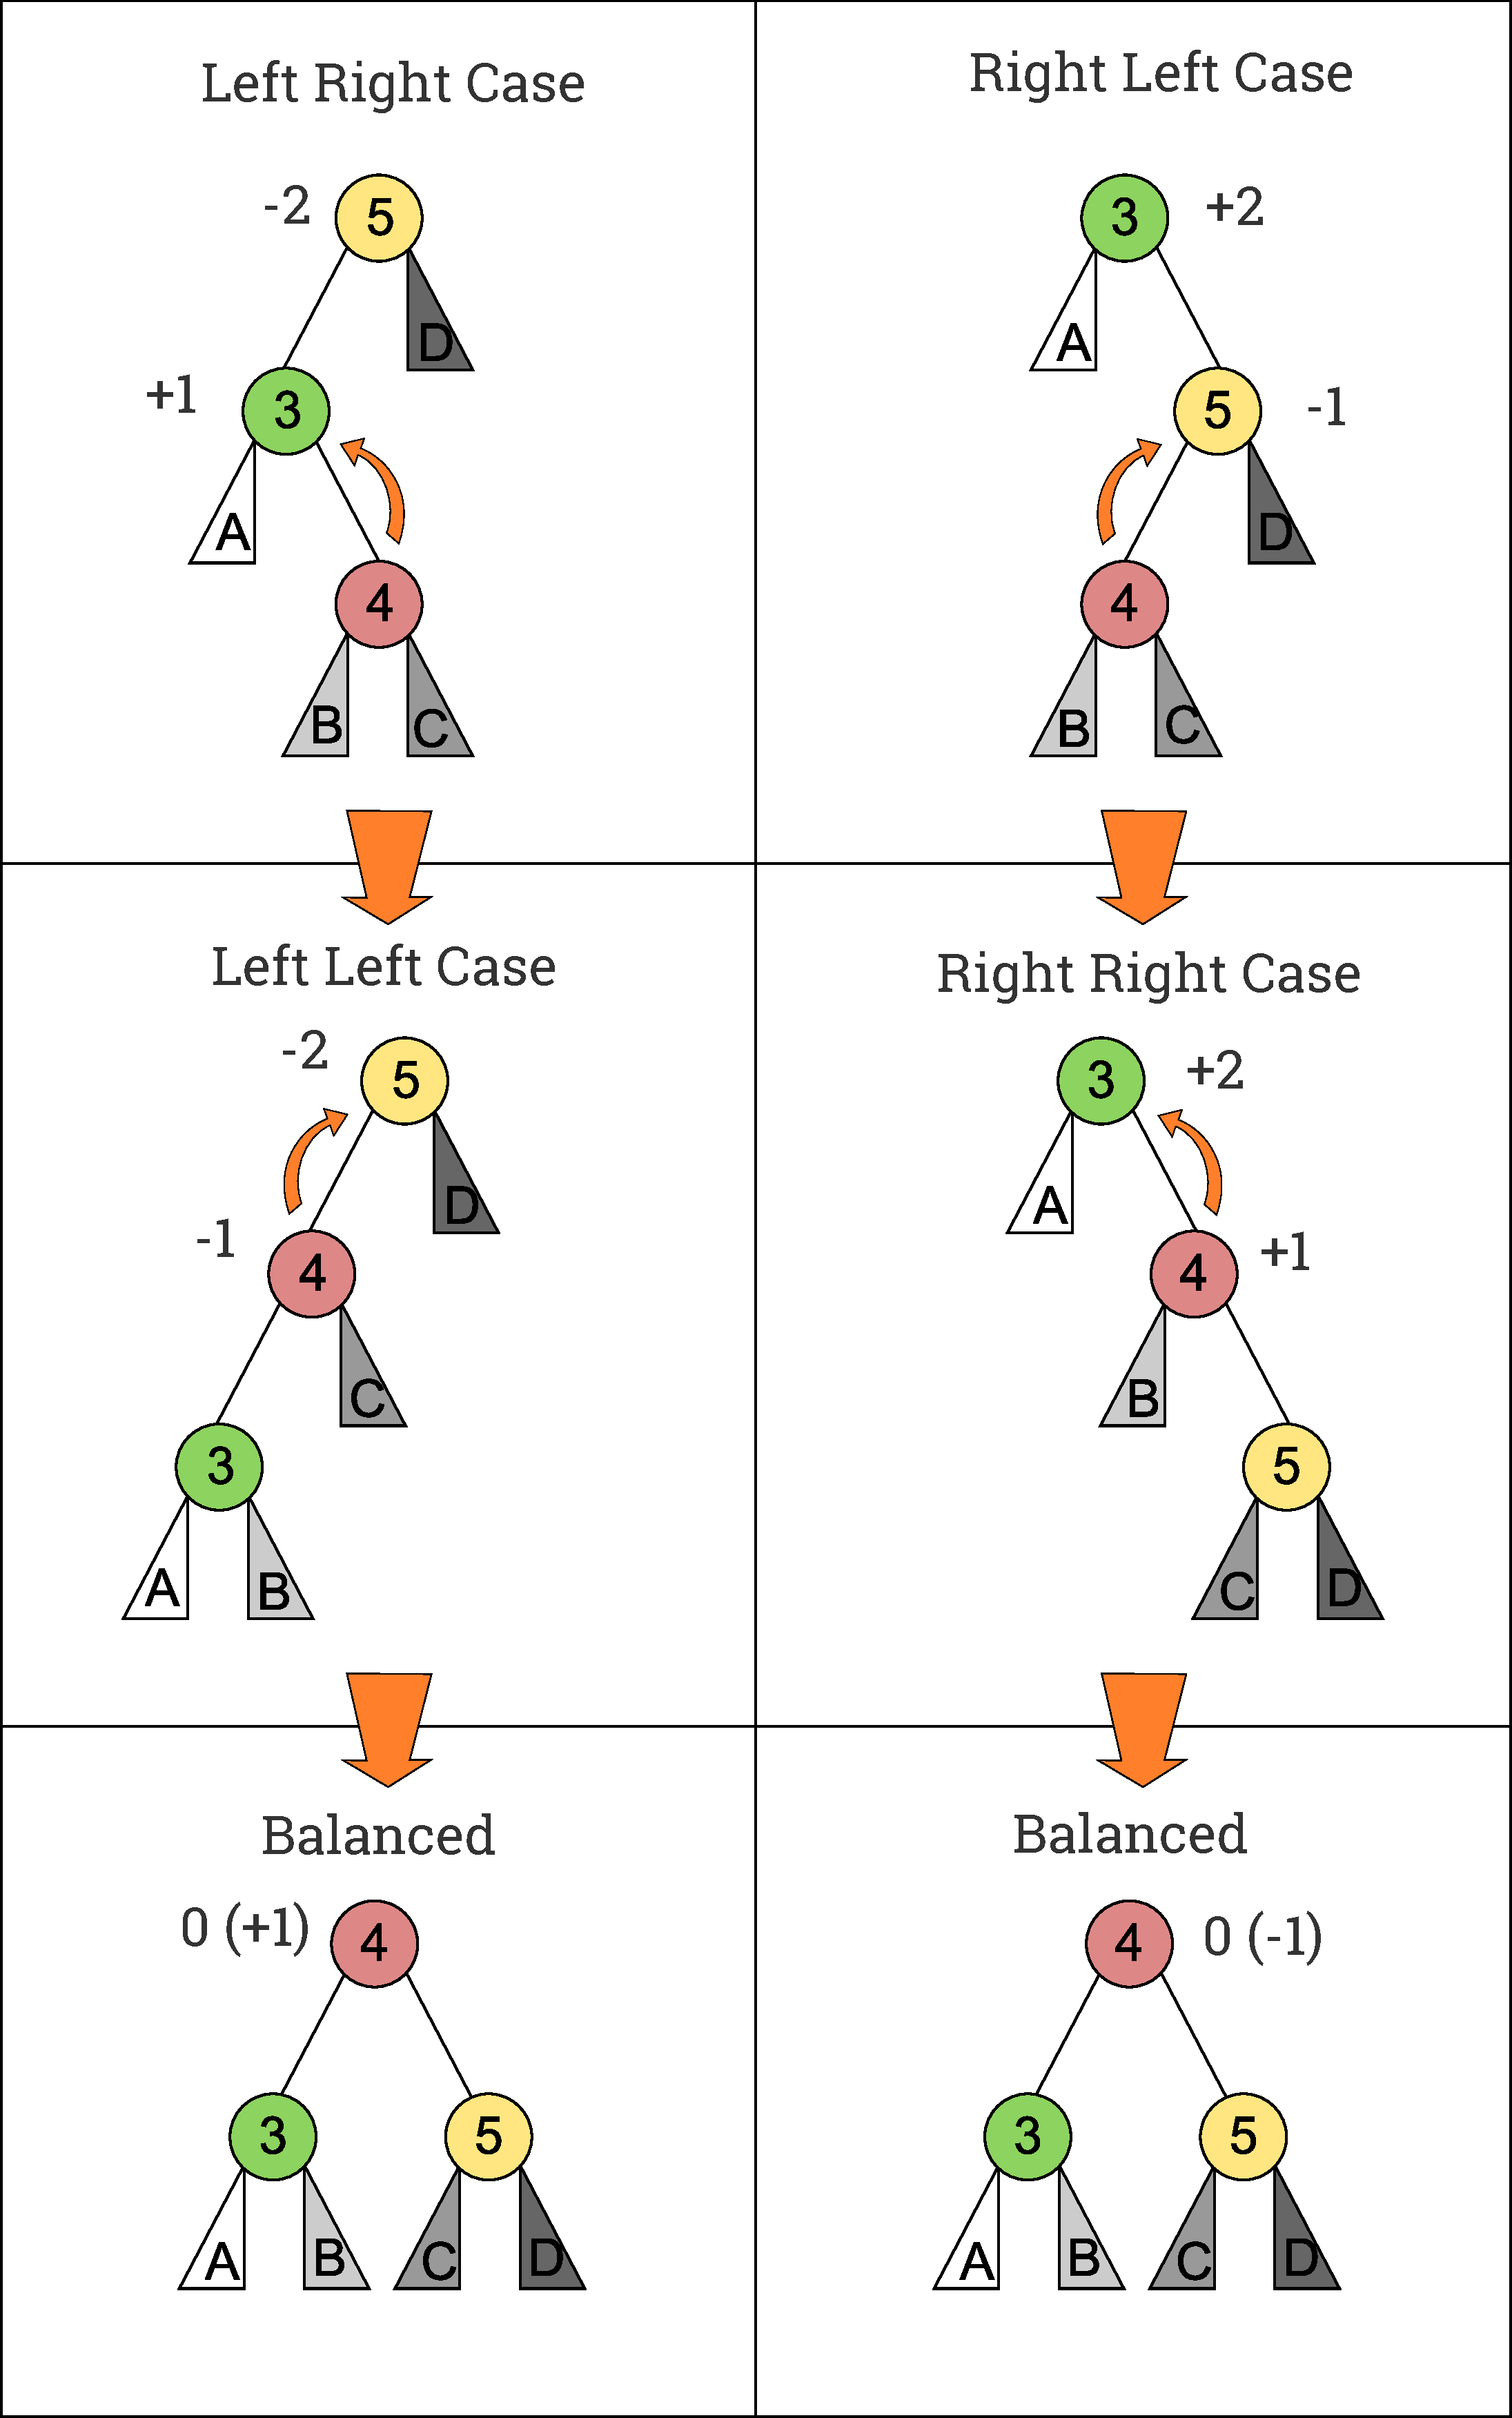
\includegraphics[width= 0.5\textwidth]{img/AVL_Tree_Rebalancing}
    \caption{Rebalancierung}
    \label{fig:AVL-Cases}
\end{figure}
\begin{figure}
    \centering
    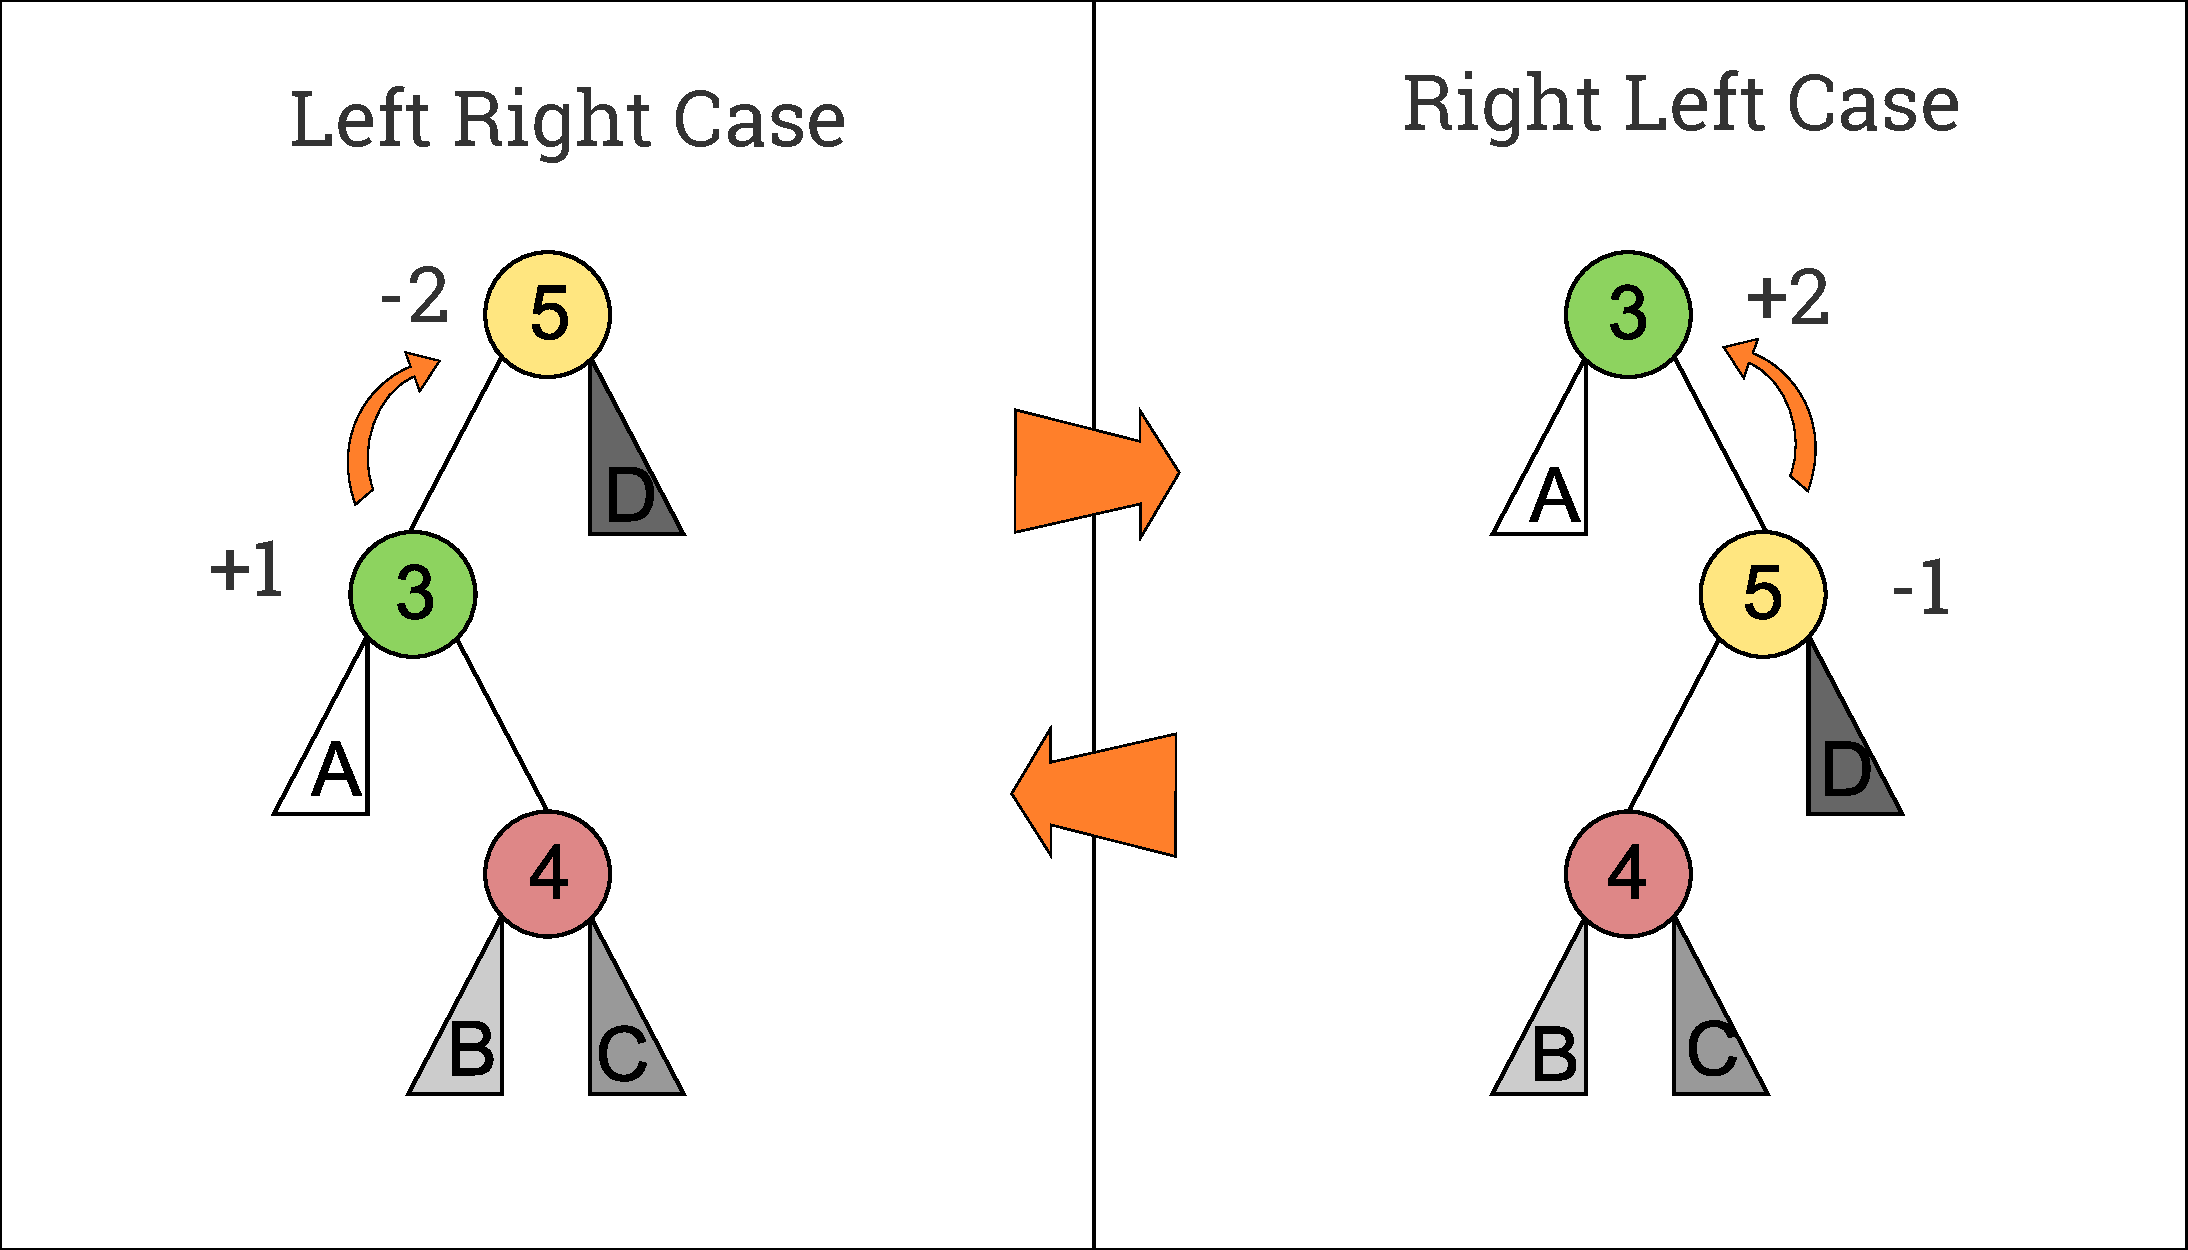
\includegraphics[width= 0.5\textwidth]{img/AVL_Tree_Rebalancing_wrong.pdf}
    \caption{Falsche Rotation}
    \label{fig:AVL-wrong-rotate}
\end{figure}

\subsection{Entwurf}\label{subsec:entwurf2}

\paragraph{InitBT, IsEmptyBT, EqualBT, FindBT}
Es müssen keine Änderungen von der ersten Praktikumsaufgabe vorgenommen werden.

\paragraph{IsBT}
Die Methode aus der ersten Praktikumsaufgabe wird um die Überprüfung der
AVL-Bedingung erweitert.
Dabei wird bei jedem Knoten überprüft, ob die Balance (siehe Formel~\ref{eq:balance}) -1, 0 oder
+1 beträgt.

\paragraph{InsertBT, DeleteBT}
Das Einfügen und Löschen wird wie bei einem Binärbaum realisiert.
Die einzige Änderung, die vorgenommen werden muss, ist das Prüfen der
AVL-Bedingung und eventuelles Rotieren, bottom-up nach dem Einfügen bzw. Löschen.
